\documentclass[12pt, addpoints]{exam/exam}

\usepackage{hyperref}
%\usepackage{mdframed}
\usepackage{graphicx, caption}	
%\usepackage{array, multicol, tabu}
\usepackage{amsmath, amsthm, amssymb}
\usepackage{comment}
\usepackage{enumitem}
\usepackage{url}
\usepackage{textcomp}
\usepackage{wrapfig}
\newcommand{\1}{^{-1}}
\newcommand{\vect}[1]{\mathbf{#1}}
\newcommand{\R}{\mathbb R}
\newcommand{\vstr}{\vspace{\stretch{1}}}
\everymath{\displaystyle}
\setlength{\parindent}{0pt}

\theoremstyle{plain}
\newtheorem{thm}{Theorem}
\newtheorem*{thm*}{Theorem}

%\printanswers
\pointformat{\bf(\thepoints)}
\pointpoints{pt}{pts}
\bonuspointformat{\bf(\thepoints)}
\bonuspointpoints{pt}{pts}

\coverfirstpageheader{\bf MATH 236 (Calculus II) \\
		Fall 2017 \\
		}
		{}
		{{Name:} \underline{\hspace{40ex}} \\
		\vspace{0.5pc}
		Thurs 16 Nov 2017}
\coverextraheadheight[2pc]{0in}
\coverfirstpagefooter{}{}{\Large Good luck!}
\coverrunningheader{}
	{Exam 3: Taylor series}
	{}
\coverrunningheadrule	
\coverrunningfootrule
\coverrunningfooter{Calc II Fall 2017}{}{p. \thepage\ (of \numpages)}

\firstpageheader{}
	{Exam 3: Taylor series}
	{}
\firstpageheadrule
\firstpagefootrule
\firstpagefooter{Calc II Fall 2017}{}{p. \thepage\ (of \numpages)}

\runningheadrule
\runningheader{}
	{Exam 3: Taylor series}
	{}
\runningfootrule
\runningfooter{Calc II Fall 2017}{}{p. \thepage\ (of \numpages)}

\title{\vspace{-8pc}
\vfill{\Huge
	\bf Exam 3: Taylor series \\ 
	(Chapter 8)} 
	}
%\author{}
\date{}

% % % % % % % % % % % % % % % % % % % %
\begin{document}

\begin{coverpages}
\maketitle
\thispagestyle{headandfoot}
\vspace{-4pc}
{\bf Exam Instructions:} You have 75 minutes to complete this exam.  Justification is required for all problems.  Notation matters!  You will also be penalized for missing units and rounding errors.  
No electronic devices (phones, iDevices, computers, etc) except for a \textbf{basic scientific calculator}.  On story problems, round to two decimal places. 

\vspace{1pc}
If you finish early then you may leave, UNLESS there are less than 5 minutes of class left.  To prevent disruption, if you finish with less than 5 minutes of class remaining then please stay seated and quiet.

\begin{flushright}
%In addition, please provide the following data:

\vspace{0.3in}
%Drill Instructor: \underline{\hspace{40ex}}

\vspace{0.3in}
%Drill Time: \underline{\hspace{40ex}}
\end{flushright}

\vfill
\textbf{Your signature below indicates that you have read this page and agree to follow the Academic Honesty Policies of James Madison University.}  

\vspace{0.3in}
Signature: {\bf (1 pt)} \underline{\hspace{73ex}}

% % % % % % % % % %
\newpage
\textbf{Formulas you may need:}
\vspace{0.5pc}

$
\begin{array}{r c l c}
%\begin{tabular}{c | c | c}
%\text{\bf Function} & \text{\bf Series} & \text{\bf Int. of Conv.} \\
\sin x &=& \sum_{k=0}^{\infty}\frac{(-1)^k}{(2k+1)!}x^{2k+1} & \text{ for }x\in\R \\
\cos x &=& \sum_{k=0}^{\infty}\frac{(-1)^k}{(2k)!}x^{2k} & \text{ for }x\in\R \\
e^x &=& \sum_{k=0}^{\infty}\frac{1}{k!}x^k & \text{ for }x\in\R \\
\frac{1}{1-x} &=& \sum_{k=0}^{\infty}x^k & \text{ for }x\in(-1,1) \\
\ln(1+x) &=& \sum_{k=1}^{\infty}\frac{(-1)^{k+1}}{k}x^k & \text{ for }x\in\left(-1,1\right] \\
\arctan x &=& \sum_{k=0}^{\infty}\frac{(-1)^k}{2k+1}x^{2k+1} & \text{ for }x\in[-1,1] \\
\sinh x &=& \sum_{k=0}^{\infty}\frac{1}{(2k+1)!}x^{2k+1} & \text{ for }x\in\R \\
\cosh x &=& \sum_{k=0}^{\infty}\frac{1}{(2k)!}x^{2k} & \text{ for }x\in\R \\
(1+x)^p &=& 1+\sum_{k=1}^{\infty}\frac{p(p-1)\cdots(p-k+1)}{k!}x^k & \\
 &=& \sum_{k=0}^{\infty}\binom{p}{k}x^k & \text{ for }x\in(-1,1)^*
\end{array}
$

$^*$The endpoints may or may not be included, depending on $p$.  You will have to check in each case.
%
%\end{tabular}

\vspace*{\fill}

\vfill
%\gradetable

\vspace{-2pc}
%\begin{center}
%\vspace*{\fill}
%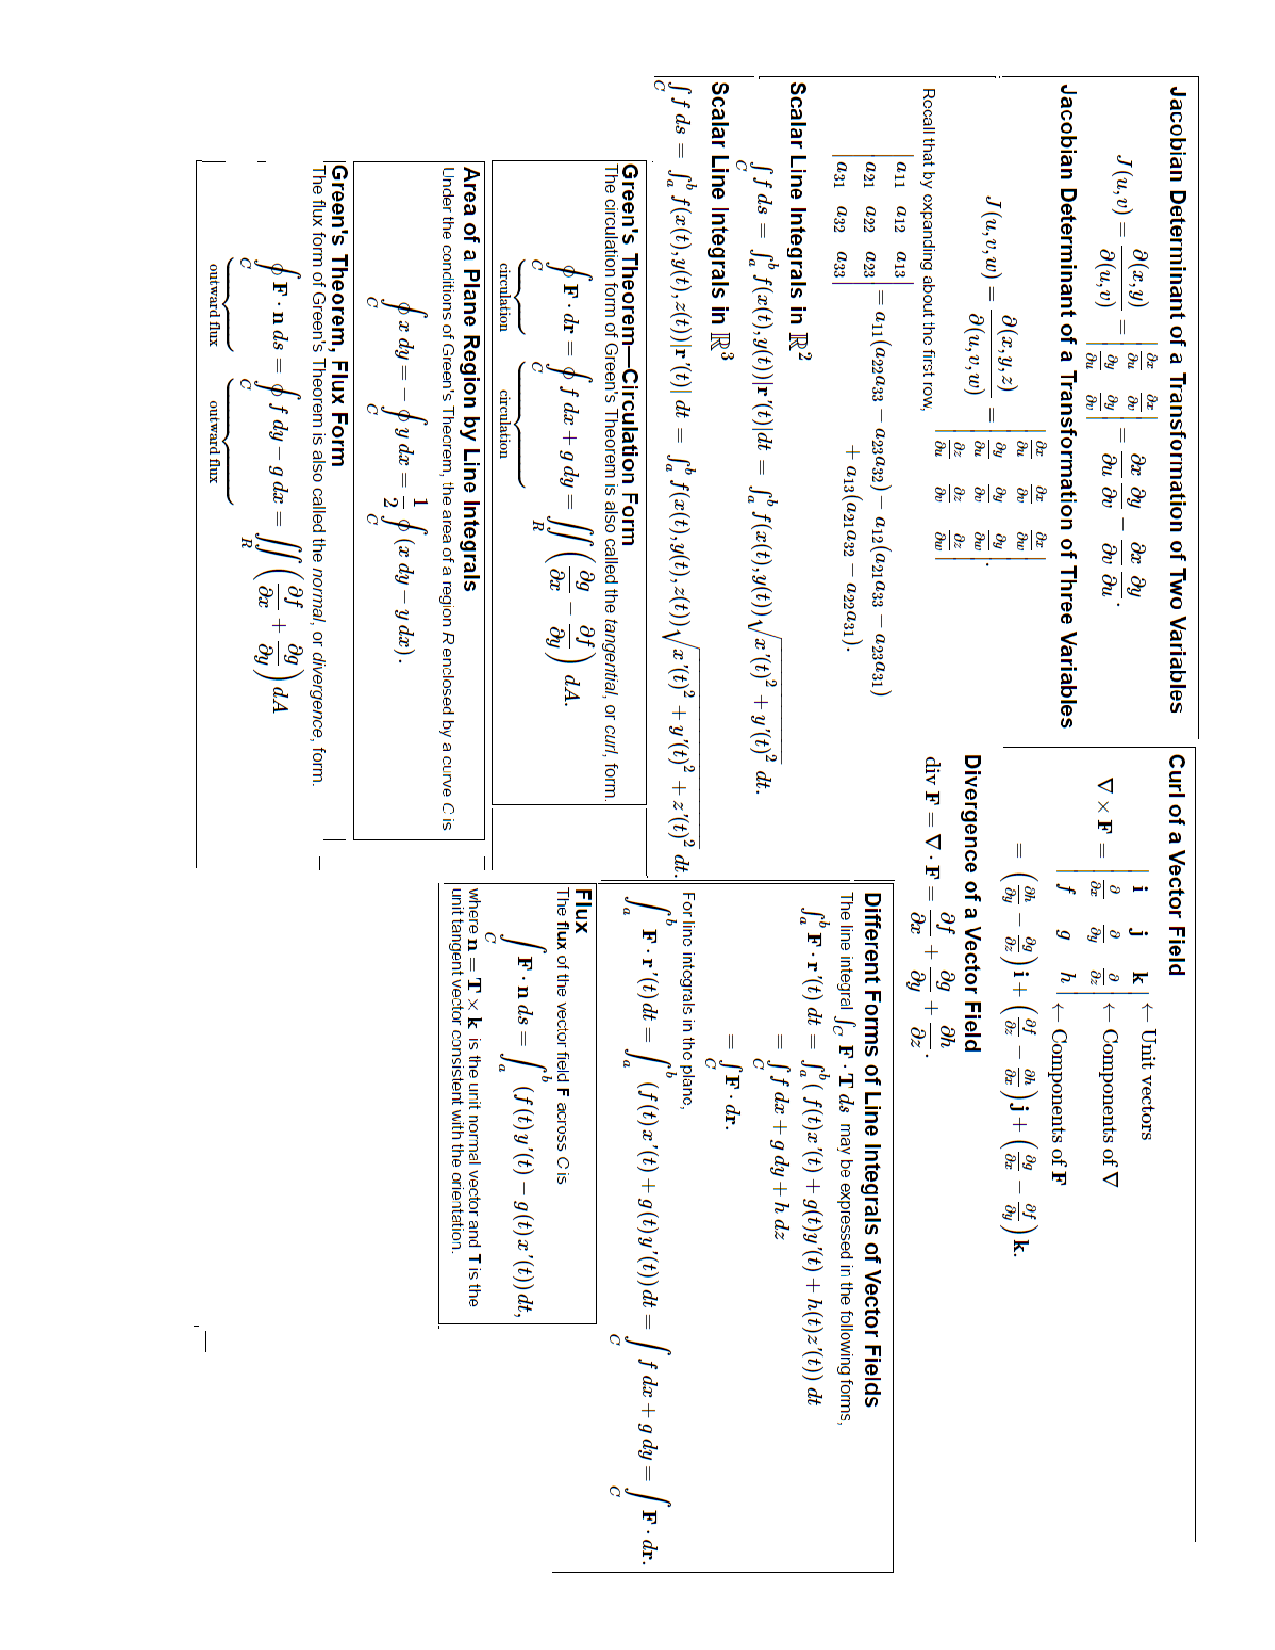
\includegraphics[scale=0.84]{Exam3FormulaSheet.pdf}
%\vspace*{\fill}
%\end{center}
\end{coverpages}

% % % % % % % % % % % % % % % % % % % %
\begin{questions}
\thispagestyle{headandfoot}

% % % % %
\question[] %{\bf 8.4 \#10}
 If $f$ is a function such that $f(0)=-3$ and $f'(x)=2f(x)$ for every value of $x$, find the Maclaurin series for $f$.

%\vfill

%\newpage
% % % % % 
\question[] %{\bf 8.4 \#42} 
Suppose $F'(x)=x\cos(x^3)$ and $F(0)=-1$.  Use a Maclaurin series to find $F(x)$.

%\newpage
% % % % %
\question[] %{\bf 8.3 \#62}
 Find the first five non-zero terms of the Maclaurin series for $f(x)=e^x\cos x$.
	
%\newpage
% % % % %
\question[] %{\bf 8.3 \#38} 
Use the Maclaurin series for $e^x$, to find the Taylor series for $e^x$ centered at $x=1$.  \textit{Hint: $\textstyle e^{x-1}=\frac{1}{e}e^x$.}

%\newpage
% % % % %
\question[] %{\bf 8.3 \#20} 
 Find the sum of the series $\sum_{k=1}^{\infty}\frac{(-1)^k}{k}\left(\frac{1}{\pi}\right)^k$.

%\newpage
% % % % %
\question[]% {\bf 8.1 \#44}  
Find the interval of convergence for the power series 
\[
\sum_{k=0}^{\infty}\frac{(-1)^k}{(2k+1)!}(3x+7)^{2k+1}.
\]

\end{questions}

\end{document}